\documentclass[11pt]{article}

\usepackage[margin=1in]{geometry}
\usepackage{booktabs}
\usepackage{longtable}
\usepackage{array}
\usepackage{xcolor}
\usepackage{amsmath}
\usepackage{amssymb}
\usepackage{pifont}
\usepackage{graphicx}
\usepackage{float}          % [H] placement so diagnostics sit with their source
\usepackage{tcolorbox}
\usepackage{url}            % provides \path (breakable monospace file paths)
\Urlmuskip=0mu plus 1mu     % let \url stretch/break a little more freely
\usepackage[hidelinks]{hyperref}
\usepackage{enumitem}

\tcbuselibrary{skins,breakable}

% ---- dynamic numbers (filled from the actual build by fill_numbers.py) -------
\newcommand{\NBG}{5,187}              % Bay Area block groups
\newcommand{\NJURIS}{188}           % distinct jurisdictions
\newcommand{\NMAPUNITS}{1,650}        % SSURGO map units
\newcommand{\NSURVEY}{11}            % SSURGO survey areas (12 county overlaps; CA689 spans SF+San Mateo)
\newcommand{\NPUMASBA}{73}         % Bay Area PUMAs
\newcommand{\NPUMSHH}{795,209}          % CA PUMS household records
\newcommand{\NPUMSHHBA}{193,449}        % of which Bay Area
\newcommand{\NTOTJOBS}{4,015,993}         % total LODES jobs (BA)
\newcommand{\NSOILPOLY}{39,021}           % SSURGO mapunit polygons
\newcommand{\NSOILBG}{5,184}             % BGs with soil coverage
\newcommand{\NSOILCOV}{99.7\%}            % mean BG soil coverage fraction
\newcommand{\NSTOPS}{21,028}              % 511 regional GTFS stops (all operators)
\newcommand{\NTRANSITBG}{4,590}          % BGs with transit (all-operator measure)
\newcommand{\NTRANSITBGBC}{713}        % BGs with transit (BART+Caltrain baseline)
% CoreLogic / Cotality
\newcommand{\CLNTX}{5,337,067}               % CoreLogic transactions
\newcommand{\CLNPARCEL}{2,275,275}           % CoreLogic parcels
\newcommand{\CLNRESPARCEL}{1,908,377}        % residential parcels
\newcommand{\CLNANALYSIS}{3,169,205}         % analysis-subset transactions
\newcommand{\CLGEORATE}{99.9\%}           % transactions geocoded to a BG
\newcommand{\CLMATCHRATE}{100.0\%}         % transactions matched to a parcel
\newcommand{\CLYEARMIN}{1900}
\newcommand{\CLYEARMAX}{2024}
\newcommand{\ZONEN}{87,329}             % zoning parcels (9-county)
\newcommand{\ZONECODES}{4,725}          % distinct zoning codes
\newcommand{\NSCHOOLS}{1,720}           % Bay Area schools
\newcommand{\CRIMEN}{1,389,347}           % SF crime incidents geocoded
\newcommand{\CRIMEBG}{1,068}              % SF BGs with crime
\newcommand{\TOTALSIZE}{1.5\,GB}        % total bytes pulled

% ACTION REQUIRED box
\newtcolorbox{actionbox}[1]{breakable, colback=red!4, colframe=red!60!black,
  fonttitle=\bfseries, title={ACTION REQUIRED --- #1}}
% RECEIVED box (a manual source that has since landed)
\newtcolorbox{receivedbox}[1]{breakable, colback=green!4, colframe=green!45!black,
  fonttitle=\bfseries, title={RECEIVED --- #1}}

\newcommand{\role}[1]{\textit{Layer~I role:} #1}

\title{\textbf{Demand-Side Data Collection:\\ Sources, Provenance, and Manual Hand-offs}}
\author{Daniel Posthumus}
\date{Generated 2026-06-12 \\ \texttt{market-for-housing-regulation} --- Layer~I}

\begin{document}
\maketitle
\tableofcontents
\bigskip

% =============================================================================
\section{Overview}
% =============================================================================
This report documents the automated acquisition of the \emph{demand-side} data
inputs for Layer~I (housing-demand estimation), covering the nine-county ABAG
Bay Area (FIPS \texttt{06001, 06013, 06041, 06055, 06075, 06081, 06085, 06095,
06097}). The data are \emph{region-wide} (not per-locality) and therefore live
at the Dropbox data root under \texttt{data/demand/}, resolved through the
repository's existing \texttt{paths.py}/\texttt{MFHR\_DATA\_ROOT} convention; the
collection code lives in \texttt{demand\_estimation/}. Of the twelve data
sources, ten are \textbf{fully automated} here (ACS PUMS and aggregate tables,
LEHD LODES8, TIGER/Line, USDA SSURGO, CGS seismic hazard, Gov-OPR statewide
zoning, CPAD open space, CDE schools, GTFS transit, and IRS migration). Two are
licensed and could not be automated: \textbf{CoreLogic} (the price/transaction
spine) and \textbf{RS Means} (the construction-cost schedule that turns the soil
instrument into a predicted-cost index). \textbf{CoreLogic has since been pulled
manually and processed} (Section~\ref{sec:corelogic}); \textbf{RS Means is now
the single outstanding manual blocker} (Section~\ref{sec:manual}). A third item,
Infutor/Verisk migration, is an optional licensed upgrade for which a free IRS
backup was pulled automatically.

Every fetch is idempotent, checksummed, and logged to
\path{data/demand/_manifest.csv}. In total \TOTALSIZE{} was pulled across the
automated sources.

% =============================================================================
\section{Automated sources (inventory)}
% =============================================================================
Table~\ref{tab:inventory} is the source inventory: one row per automated source,
with counts, sizes, and statuses read directly from the manifest. Status
\texttt{downloaded}/\texttt{cached}/\texttt{verified} means data is present;
\texttt{needs\_key} means automatable but pending a credential;
\texttt{partial} means some artifacts of a multi-part source landed. (USDA SSURGO
appears as two rows --- the tabular engineering extract and the spatial polygons
that join it to block groups.)

\begin{center}
\scriptsize
\setlength{\tabcolsep}{3pt}
\renewcommand{\arraystretch}{1.15}
\begin{longtable}{p{1.7cm} p{2.6cm} p{1.45cm} p{1.5cm} p{2.45cm} c p{1.05cm} p{1.55cm} p{0.7cm}}
\caption{Automated demand-side source inventory (from \texttt{\_manifest.csv}).}
\label{tab:inventory}\\
\toprule
Source & Layer-I role & Vintage & Access & Endpoint & \# & Size & Status & Chk\\
\midrule
\endfirsthead
\multicolumn{9}{l}{\emph{(Table~\ref{tab:inventory} continued)}}\\
\toprule
Source & Layer-I role & Vintage & Access & Endpoint & \# & Size & Status & Chk\\
\midrule
\endhead
\midrule
\multicolumn{9}{r}{\emph{continued\ldots}}\\
\endfoot
\bottomrule
\endlastfoot
ACS 5-yr PUMS & Household micro-data (BLP random-coefficient moments) & 2020--2024 ACS 5-yr & FTP bulk (keyless) & \url{www2.census.gov/programs-surveys/acs/data/pums/2024/5-Year} & 2 & 350.4\,MB & cached & sha256 \\
ACS aggregate tables & Tract/BG shares: tenure, value, rent, income, structure & 2023 ACS 5-yr & Census Data API (key) & \url{api.census.gov/data/2023/acs/acs5} & 2 & 697.6\,KB & cached & n/a \\
LEHD LODES8 & Job access $JA_\ell$ (agglomeration coupling) & LODES8 v8.3 (2022, 2015) & direct download & \url{lehd.ces.census.gov/data/lodes/LODES8/ca} & 7 & 135.3\,MB & cached, downloaded & sha256 \\
TIGER/Line geography & Geography spine; BG$\leftrightarrow$jurisdiction overlay & TIGER2023 & direct download & \url{www2.census.gov/geo/tiger/TIGER2023} & 5 & 176.0\,MB & cached & sha256 \\
USDA SSURGO (tabular) & \textbf{Instrument}: shrink-swell/plasticity/bearing (mukey) & SDA current (2025 saverest) & Soil Data Access REST & \url{sdmdataaccess.sc.egov.usda.gov/Tabular/post.rest} & 12 & 2.1\,MB & cached, downloaded & sha256 \\
SSURGO (spatial) & Mapunit polygons --- the mukey$\to$BG join & SDA current & Soil Data Access REST & \url{sdmdataaccess.sc.egov.usda.gov/Tabular/post.rest} & 11 & 196.6\,MB & cached & sha256 \\
CGS seismic hazard & Instrument \emph{control} (seismic capitalization) & CGS current & ArcGIS Feature Service & \url{services2.arcgis.com/Geohazards} & 2 & 22.3\,MB & cached & sha256 \\
Gov-OPR statewide zoning & By-right envelope backstop (Layer II) & 2022--23 snapshot & ArcGIS Feature Service & \url{services8.arcgis.com/California_Statewide_Zoning_North} & 1 & 453.1\,MB & cached & sha256 \\
CPAD open space & Amenity \emph{control} (proximity to protected areas) & CPAD 2024a & ArcGIS Feature Service & \url{services1.arcgis.com/cpad_2024a_unitsgdb} & 1 & 32.4\,MB & cached & sha256 \\
CDE schools & Amenity: school enrollment / quality proxy & CDE current & bulk flat file & \url{www3.cde.ca.gov/demo-downloads/ce/cenroll2324.txt} & 1 & 19.3\,MB & cached & sha256 \\
GTFS transit & Amenity: transit access (all operators via 511) & 511 + agency current & 511 API + per-agency & \url{api.511.org/transit/datafeeds} & 3 & 77.7\,MB & cached, downloaded & sha256 \\
IRS SOI migration & Moving-cost backup (free; Infutor/Verisk upgrade) & 2021--2022 & direct download & \url{irs.gov/pub/irs-soi/countyinflow2122.csv} & 2 & 8.5\,MB & cached & sha256 \\
Crime (SF+Oak+FBI) & Location disamenity: incident BG (SF, Oakland) + FBI county & 2019--24; FBI 2022 & Socrata + FBI CDE + geocoder & \url{data.sfgov.org; api.usa.gov/crime/fbi} & 4 & 9.7\,MB & cached, downloaded & sha256 \\

\end{longtable}
\end{center}

% =============================================================================
\section{Dataset granularity \& key fields}
% =============================================================================
Table~\ref{tab:grain} states, for every dataset, its \emph{unit of observation}
(the grain at which each row sits) and the key fields carried, so it is explicit
what information each source contributes and at what level it must be aggregated
to reach the block-group estimation geography.

\begin{center}
\footnotesize
\setlength{\tabcolsep}{4pt}
\renewcommand{\arraystretch}{1.2}
\begin{longtable}{p{2.5cm} p{3.3cm} p{8.4cm}}
\caption{Granularity (unit of observation) and key fields by dataset.}
\label{tab:grain}\\
\toprule
Dataset & Grain (unit of obs.) & Key fields \\
\midrule
\endfirsthead
\toprule
Dataset & Grain (unit of obs.) & Key fields \\
\midrule
\endhead
\bottomrule
\endfoot
\bottomrule
\endlastfoot
ACS PUMS (housing) & household record (weighted) & \texttt{TEN, HINCP, VALP, RNTP, BDSP, NP, BLD, YRBLT}; \texttt{PUMA}, \texttt{bay\_area} flag \\
ACS PUMS (person) & person record (weighted) & \texttt{AGEP, RAC1P, SCHL, HISP, SEX}; \texttt{PUMA} \\
ACS tables & block group \& tract & tenure / value / rent / income / structure counts (8 table groups), keyed by \texttt{GEOID} \\
LEHD LODES8 & workplace block $\to$ block group & jobs by block (\texttt{C000}); distance-decay job access $JA_\ell$ \\
TIGER/Line & polygons: county, tract, BG, place, PUMA & \texttt{GEOID}, \texttt{geometry}; the BG$\leftrightarrow$jurisdiction crosswalk \\
SSURGO (tabular) & map unit (\texttt{mukey}) $\times$ soil horizon & \texttt{lep\_r} (shrink-swell), \texttt{pi\_r}, \texttt{ll\_r}, $K_{sat}$, drainage, taxonomy \\
SSURGO (spatial) & map-unit polygon & \texttt{mukey}, \texttt{geometry}; areal weights to block groups \\
CGS hazard & hazard-zone polygon & seismic / liquefaction zones, Alquist--Priolo fault traces $\to$ BG area share \\
Gov-OPR zoning & zoning polygon (parcel-level) & \texttt{County}, \texttt{Jurisdiction}, zoning \texttt{Code} \\
CPAD open space & protected-area polygon & access type, managing agency $\to$ BG distance to nearest \\
CDE schools & school $\times$ year & cumulative enrollment by school \\
GTFS transit & transit stop & \texttt{stop\_lat}, \texttt{stop\_lon} $\to$ BG stop density (1\,km) \\
IRS migration & county-pair $\times$ year & inflow / outflow returns, exemptions, AGI \\
Crime & incident $\to$ BG (SF, Oakland); county (FBI, all 9) & SF/Oakland incidents geocoded to BG; FBI violent+property county rate per 100k \\
CoreLogic deed & transaction (recorded sale) & \texttt{SALE\_AMOUNT}, \texttt{SALE\_DERIVED\_DATE}, deed/sale-type codes, resale/new-construction/interfamily/REO indicators \\
CoreLogic property & parcel (\texttt{CLIP}) & land use, parcel lat/long, assessed land/improvement/total value, tax, beds/baths/rooms, living \& lot sq ft, units, stories, foundation, owner-occupancy \\
\end{longtable}
\end{center}

% =============================================================================
\section{Per-source detail}
% =============================================================================

\subsection{ACS 5-year PUMS (household micro-data)}
The household side of BLP. Downloaded via the \emph{keyless} Census FTP bulk path
(\texttt{csv\_hca.zip} housing + \texttt{csv\_pca.zip} person, California,
2020--2024 5-year), so no API key is required. The build identifies the
\NPUMASBA{} 2020 PUMAs intersecting the nine counties (spatial join of the TIGER
PUMA20 layer against the county layer) and tags each CA record with a
\texttt{bay\_area} flag, writing \path{ca_pums_household.parquet}
(\NPUMSHH{} records; \NPUMSHHBA{} Bay Area) and \path{ca_pums_person.parquet}.
Variables retained: \texttt{TEN, HINCP, VALP, RNTP, BDSP, NP, BLD, YRBLT}
(housing) and \texttt{AGEP, RAC1P, SCHL, HISP, SEX} (person), plus
\texttt{PUMA, ST, SERIALNO} and the survey weights \texttt{WGTP}/\texttt{PWGTP}.
All moments below are \textbf{\texttt{WGTP}-weighted}, hence population-correct
(the weighted household total is 3.3\,M, matching the nine-county count).

\begin{table}[H]\centering\footnotesize\setlength{\tabcolsep}{5pt}
\caption{ACS PUMS household summary (Bay Area; \texttt{WGTP}-weighted).}
\label{tab:pums}\begin{tabular}{lrrrrr}
\toprule
Variable & Households (wtd) & Median & Mean & P10 & P90 \\
\midrule
Household income (HINCP) & 3,275,379 & \$115,000 & \$166,064 & \$22,200 & \$360,000 \\
Home value, owners (VALP) & 1,877,800 & \$900,000 & \$1,170,785 & \$350,000 & \$2,100,000 \\
Gross rent, renters (RNTP) & 1,350,137 & \$2,000 & \$2,209 & \$800 & \$3,700 \\
Bedrooms (BDSP) & 3,324,794 & 3 & 2.7 & 1 & 4 \\
Household size (NP) & 3,275,379 & 2 & 2.6 & 1 & 5 \\
\midrule
Owner-occupied & \multicolumn{4}{r}{57.3\% of occupied} \\
Renter-occupied & \multicolumn{4}{r}{42.7\% of occupied} \\
\bottomrule
\end{tabular}

\end{table}
\begin{figure}[H]\centering
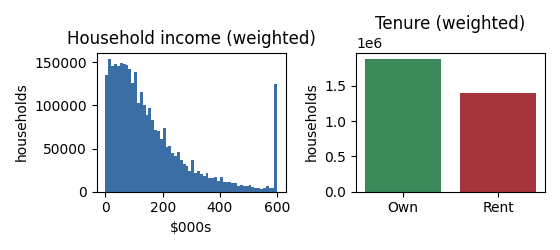
\includegraphics[width=0.85\textwidth]{figures/src_pums.png}
\caption{PUMS Bay Area households (weighted): income distribution (left) and tenure (right).}
\label{fig:pums}
\end{figure}

\subsection{ACS aggregate tables}
Tract- and block-group-level tenure, value, rent, income, and structure --- the
market shares and outside-option denominators of demand --- pulled from the
Census Data API (2023 ACS 5-year) for all nine counties: groups \texttt{B25003}
(tenure), \texttt{B25077} (value), \texttt{B25064} (rent), \texttt{B19013}
(income), \texttt{B25024} (units in structure), \texttt{B25118} (tenure by
income), \texttt{B25034} (year built), \texttt{B25040} (heating fuel). The key
is resolved from the environment / \texttt{CENSUS\_API\_KEY.txt}; if absent or
rejected the step degrades to \texttt{needs\_key} without blocking the run.

\begin{table}[H]\centering\footnotesize\setlength{\tabcolsep}{5pt}
\caption{ACS block-group aggregates (distribution across block groups).}
\label{tab:acsbg}\begin{tabular}{lrrrrr}
\toprule
Across block groups & N & Median & Mean & P10 & P90 \\
\midrule
Owner-occupancy share (\%) & 5,163 & 63.2\% & 58.3\% & 16.6\% & 91.8\% \\
Median home value & 4,778 & \$1,112,500 & \$1,175,612 & \$588,530 & \$2,000,001 \\
Median gross rent & 4,260 & \$2,600 & \$2,592 & \$1,679 & \$3,501 \\
Median household income & 4,903 & \$139,063 & \$146,032 & \$72,188 & \$250,001 \\
\bottomrule
\end{tabular}

\end{table}
\begin{figure}[H]\centering
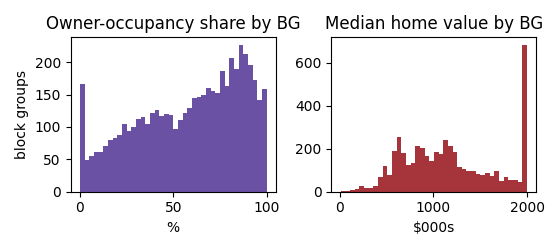
\includegraphics[width=0.85\textwidth]{figures/src_acsbg.png}
\caption{ACS block groups: owner-occupancy share (left) and median home value (right).}
\label{fig:acsbg}
\end{figure}

\subsection{LEHD LODES8 (job access)}
The agglomeration coupling: job access $JA_\ell$ is the empirical analogue of the
toy model's regional wage $w_m=w(N)$. WAC (workplace jobs by block), RAC, OD
(main+aux), and the block crosswalk for California were downloaded for the panel
year 2022 plus a 2015 pre-period for robustness. The build aggregates WAC jobs to
block groups and computes a distance-decay job-access measure
$JA_i=\sum_j W_j e^{-d_{ij}/d_0}$ ($d_0=10$\,km, great-circle between BG
centroids in CA-Albers), plus 10\,km/30\,km job counts, over the
\NBG{} Bay Area block groups ($\sum_j W_j=\NTOTJOBS$ jobs).

\begin{figure}[H]\centering
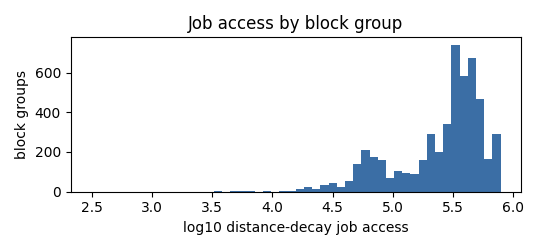
\includegraphics[width=0.58\textwidth]{figures/src_jobaccess.png}
\caption{Distance-decay job access by block group (log scale).}\label{fig:jobaccess}
\end{figure}
Table~\ref{tab:bgcov} collects the block-group covariates contributed by this and
the next few sources (LODES, SSURGO, CGS, CPAD, GTFS) in one place.
\begin{table}[H]\centering\footnotesize\setlength{\tabcolsep}{5pt}
\caption{Block-group covariate summary (LODES job access, SSURGO soil, CGS / CPAD / GTFS controls).}
\label{tab:bgcov}\begin{tabular}{lrrrrr}
\toprule
Block-group covariate & N & Median & Mean & P10 & P90 \\
\midrule
Jobs located in BG (LODES) & 5,187 & 193 & 774 & 44 & 1,363 \\
Job access (decay-weighted) & 5,187 & 326,589 & 320,037 & 60,884 & 545,295 \\
Jobs within 30 km & 5,187 & 1,415,136 & 1,186,822 & 203,833 & 1,815,310 \\
Seismic-zone area share (CGS) & 5,187 & 0 & 0.1 & 0 & 0.8 \\
Open-space distance, m (CPAD) & 5,187 & 285 & 382 & 31.3 & 749 \\
Transit stops $\leq$1\,km, all ops & 5,187 & 20 & 40.0 & 0 & 93 \\
Soil expansive share (SSURGO) & 4,075 & 0 & 0.2 & 0 & 0.9 \\
Soil linear extensibility, lep & 4,075 & 3.6 & 3.5 & 0 & 7.3 \\
\bottomrule
\end{tabular}

\end{table}

\subsection{TIGER/Line geography \& the BG$\leftrightarrow$jurisdiction crosswalk}
Counties, tracts, block groups, places, and PUMAs (TIGER2023). The single most
load-bearing derived artifact is \path{geography/crosswalks/bg_to_jurisdiction.parquet}:
each of the \NBG{} block groups is assigned to its dominant incorporated place by
areal overlap (intersection in CA-Albers; dominant place = max intersection
area), or to the ``Unincorporated \emph{County}'' remainder when no place covers
a majority of its area. This operationalizes the demand memo's design in which
jurisdiction is an \emph{attribute of the location}; \NJURIS{} distinct
jurisdictions result.

\begin{table}[H]\centering\footnotesize\setlength{\tabcolsep}{6pt}
\caption{Geography by county (block groups, jurisdictions, unincorporated BGs).}
\label{tab:geo}\begin{tabular}{lrrr}
\toprule
County & Block groups & Jurisdictions & Uninc.\ BGs \\
\midrule
Alameda & 1,134 & 21 & 18 \\
Contra Costa & 708 & 47 & 51 \\
Marin & 181 & 23 & 22 \\
Napa & 108 & 8 & 29 \\
San Francisco & 681 & 1 & 0 \\
San Mateo & 500 & 30 & 37 \\
Santa Clara & 1,173 & 25 & 48 \\
Solano & 298 & 10 & 43 \\
Sonoma & 404 & 24 & 132 \\
\midrule
\textbf{All 9 counties} & 5,187 & 188 & 380 \\
\bottomrule
\end{tabular}

\end{table}

\subsection{USDA SSURGO (the instrument)}
The cost-shifter instrument's raw material. Rather than the multi-GB gSSURGO
geodatabase, we use the USDA Soil Data Access (SDA) tabular REST service, which
returns exactly the engineering fields needed without a spatial download. The
nine counties are covered by \NSURVEY{} SSURGO survey areas (12 county overlaps;
survey CA689 spans both San~Francisco and San~Mateo), discovered at runtime from
the County-or-Parish overlap (symbols are not all FIPS-aligned ---
Alameda/SF/San~Mateo/Santa~Clara use legacy survey symbols). For each survey
area we pull \texttt{mapunit}$\,\to\,$\texttt{component}$\,\to\,$\texttt{chorizon}
linear extensibility (\texttt{lep\_r}, shrink-swell / COLE proxy), plasticity
index (\texttt{pi\_r}), liquid limit (\texttt{ll\_r}), $K_{sat}$, bulk density,
drainage class, and taxonomy. The build aggregates horizons of the dominant
component to a depth-weighted (0--150\,cm) profile, yielding
\path{soil/derived/mapunit_engineering_properties.parquet} (\NMAPUNITS{} map
units, with a derived shrink-swell class).

\paragraph{Map-unit $\to$ block-group join (now built).} The tabular SDA route
returns no geometry, so a second pull (\path{ssurgo_spatial.py}) fetches the
SSURGO spatial \texttt{MUPOLYGON} mapunit polygons --- \NSOILPOLY{} polygons
across the same \NSURVEY{} survey areas --- via SDA's WKT export, cursor-paged on
\texttt{mupolygonkey} (the public per-survey Web Soil Survey zips are not
reliably addressable without a per-survey target date; SDA is the keyless
equivalent). Polygon \texttt{mukey}s fully cover the tabular extract's mukeys.
The build areal-intersects the polygons with the block groups in CA-Albers and
writes \path{soil/derived/bg_soil_engineering.parquet}: each of the \NSOILBG{}
covered block groups carries the area-weighted \texttt{lep}/\texttt{pi}/\texttt{ll}/
\texttt{ksat}/bulk-density, the expansive (high + very-high shrink-swell) area
share, a coverage fraction, and an area-weighted missingness flag (mean coverage
\NSOILCOV{} of BG area). This resolves the BG-aggregation TODO the first run
flagged; see Section~\ref{sec:instrument} for the one remaining blocker.

\begin{figure}[H]\centering
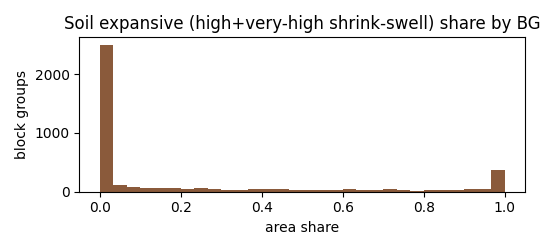
\includegraphics[width=0.58\textwidth]{figures/src_soil.png}
\caption{Soil expansive (high + very-high shrink-swell) area share by block group
--- the instrument's raw spatial variation.}\label{fig:soil}
\end{figure}

\subsection{CGS seismic hazard (control)}
Seismic risk is a \emph{control}, not an instrument: it must be partialled out so
the soil instrument is not contaminated by the seismic-capitalization channel.
The statewide CGS Seismic Hazard Zones (zones of required investigation, incl.
liquefaction and earthquake-induced landslides) feature layer is pulled clipped
to the Bay Area bounding box, alongside the public Alquist--Priolo fault traces.
The build computes each BG's share of area inside a hazard zone.

\subsection{Gov-OPR statewide zoning (Layer II backstop)}
The by-right envelope $\bar z_j$ backstop --- a single 2022--23 aggregated
statewide snapshot from the Governor's Office of Planning \& Research, North half
(which covers the Bay Area), clipped to the nine counties. This feeds Layer~II,
not Layer~I; it was grabbed now because it is cheap while pulling spatial layers.
\emph{Caveat:} a snapshot, not a panel --- flag for per-city fidelity checks.

\begin{figure}[H]\centering
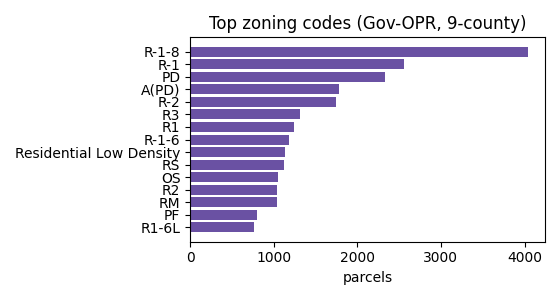
\includegraphics[width=0.6\textwidth]{figures/src_zoning.png}
\caption{Most common local zoning codes (Gov-OPR snapshot, 9-county;
\ZONEN{} parcels, \ZONECODES{} distinct codes).}\label{fig:zoning}
\end{figure}

\subsection{Amenity layers (controls)}
\textbf{Open space (CPAD 2024a)} --- like seismic, an amenity \emph{control}, so
the instrument can be residualized against proximity to protected areas; the
build computes BG-centroid distance to the nearest protected area.
\textbf{Schools (CDE)} --- enrollment flat file (school-quality / demographics
proxy), discovered from the CDE data-download page.
\textbf{Transit (GTFS).} The build counts GTFS stops within 1\,km of each BG
centroid. Two measures are kept for auditability: a keyless BART + Caltrain
baseline (\path{transit_stops_1km_bartcaltrain}, \NTRANSITBGBC{} BGs with a
stop --- essentially rail stations) and, now that a 511 Bay Area API key is
available, the full all-operator measure
(\path{transit_stops_1km_all}). The latter is built from the 511 regional
GTFS bundle (operator\_id=RG --- Muni, AC~Transit, VTA, SamTrans, and every other
operator; \NSTOPS{} stops), fetched into \path{amenities/transit/bay511/} and
unioned with the per-agency feeds: it reaches \NTRANSITBG{} BGs, a roughly
six-fold gain over the rail-only baseline. (Caltrain's standalone
\texttt{caltrain.com} feed now returns HTML, so the keyless baseline uses the
Trillium Caltrain mirror; downloads are validated as real zips before use.)

\begin{figure}[H]\centering
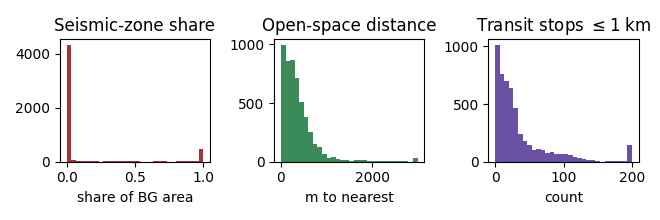
\includegraphics[width=0.97\textwidth]{figures/src_controls.png}
\caption{Instrument controls by block group: seismic-zone area share (CGS),
distance to nearest protected open space (CPAD), and transit-stop density within
1\,km (GTFS, all operators).}\label{fig:controls}
\end{figure}
\begin{figure}[H]\centering
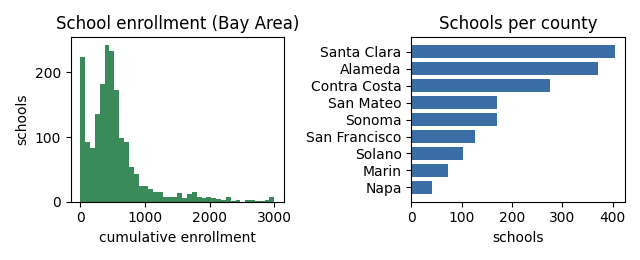
\includegraphics[width=0.85\textwidth]{figures/src_schools.png}
\caption{CDE schools: cumulative-enrollment distribution and school counts by
county (\NSCHOOLS{} Bay Area schools).}\label{fig:schools}
\end{figure}

\subsection{Crime (location disamenity)}
Crime is a classic location (dis)amenity in housing demand --- a willingness-to-pay
shifter and a control. Coverage is assembled in two layers:
\begin{itemize}[leftmargin=1.5em, itemsep=1pt]
\item \textbf{Incident-level, geocoded to block group:} San~Francisco PD
  (DataSF / Socrata, with coordinates) and Oakland PD (data.oaklandca.gov,
  addresses geocoded via the free Census batch geocoder) --- \CRIMEN{} incidents
  2019--2024 across \CRIMEBG{} block groups, written to
  \path{crime/bg_crime.parquet} as \texttt{crime\_per\_1k\_hh\_yr}.
\item \textbf{County-level, all nine counties (full coverage):} the FBI Crime
  Data Explorer (api.data.gov key) --- violent + property offenses summed over
  every agency in each county yield a rate per 100k
  (Table~\ref{tab:crime}), broadcast to every block group as
  \texttt{county\_crime\_rate\_per\_100k}.
\end{itemize}
Both layers are merged into the controls. San~Jose's only open feed is ``calls
for service'' (police activity, not crime reports) behind a portal interstitial,
so San~Jose is covered by the FBI Santa~Clara county rate rather than
incident-level. The rankings are as expected --- San~Francisco and Alameda
(Oakland) highest, Sonoma/Napa/Marin lowest.

\begin{table}[H]\centering\footnotesize\setlength{\tabcolsep}{6pt}
\caption{County crime rates (FBI CDE, 2022): violent + property offenses per 100k.}
\label{tab:crime}\begin{tabular}{lrrr}
\toprule
County (FBI 2022) & Violent & Property & Rate/100k \\
\midrule
San Francisco & 5,455 & 48,771 & 7,091 \\
Alameda & 11,022 & 68,638 & 4,918 \\
Solano & 2,506 & 12,047 & 3,229 \\
Santa Clara & 7,426 & 48,086 & 3,011 \\
Contra Costa & 4,789 & 24,528 & 2,530 \\
San Mateo & 2,291 & 15,685 & 2,514 \\
Marin & 646 & 4,449 & 1,968 \\
Napa & 453 & 2,049 & 1,854 \\
Sonoma & 1,581 & 5,791 & 1,523 \\
\bottomrule
\end{tabular}

\end{table}
\begin{figure}[H]\centering
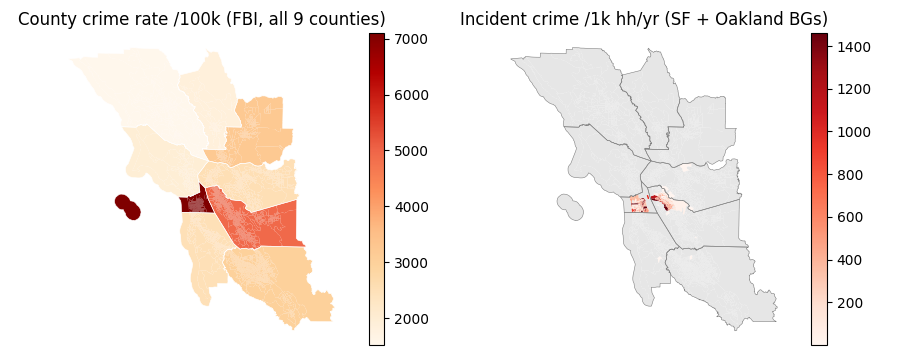
\includegraphics[width=0.95\textwidth]{figures/src_crime.png}
\caption{Crime by block group: county rate per 100k (FBI, all nine counties ---
full coverage, left) and incident crime per 1,000 households/year (SF + Oakland
block groups, right).}\label{fig:crime}
\end{figure}

\subsection{IRS migration (moving-cost backup)}
IRS SOI county-to-county inflow/outflow (2021--2022), the free automatable
first-pass moving-cost input, filtered to the nine counties. The licensed
Infutor/Verisk upgrade is stubbed (Section~\ref{sec:manual}). Every Bay Area
county except Solano shows net domestic out-migration in 2021--22 --- the
documented post-pandemic pattern.

\begin{table}[H]\centering\footnotesize\setlength{\tabcolsep}{6pt}
\caption{IRS county migration, 2021--22 (tax returns).}\label{tab:irs}\begin{tabular}{lrrr}
\toprule
County & In-returns & Out-returns & Net \\
\midrule
Alameda & 40,374 & 51,822 & -11,448 \\
Contra Costa & 24,234 & 28,095 & -3,861 \\
Marin & 5,135 & 6,044 & -909 \\
Napa & 2,293 & 2,576 & -283 \\
San Francisco & 31,061 & 35,504 & -4,443 \\
San Mateo & 20,241 & 24,779 & -4,538 \\
Santa Clara & 41,725 & 53,787 & -12,062 \\
Solano & 9,739 & 9,617 & +122 \\
Sonoma & 7,954 & 7,993 & -39 \\
\midrule
\textbf{All 9 counties} & 182,756 & 220,217 & -37,461 \\
\bottomrule
\end{tabular}

\end{table}
\begin{figure}[H]\centering
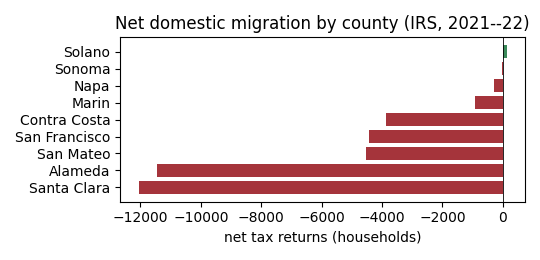
\includegraphics[width=0.6\textwidth]{figures/src_irs.png}
\caption{Net domestic migration by county (IRS SOI, 2021--22).}\label{fig:irs}
\end{figure}

\subsection{Spatial patterns}\label{sub:spatial}
Figure~\ref{fig:maps} maps the key block-group variables. The expensive
peninsula / San~Francisco / Marin core, the San~Francisco + Silicon Valley
job-access peaks (the agglomeration centre), the low-ownership rental cores, and
--- importantly for identification --- the soil instrument's \emph{independent}
spatial variation (inland and east-bay expansive clays, not aligned with the
price/income gradient) are all visible.
\begin{figure}[H]\centering
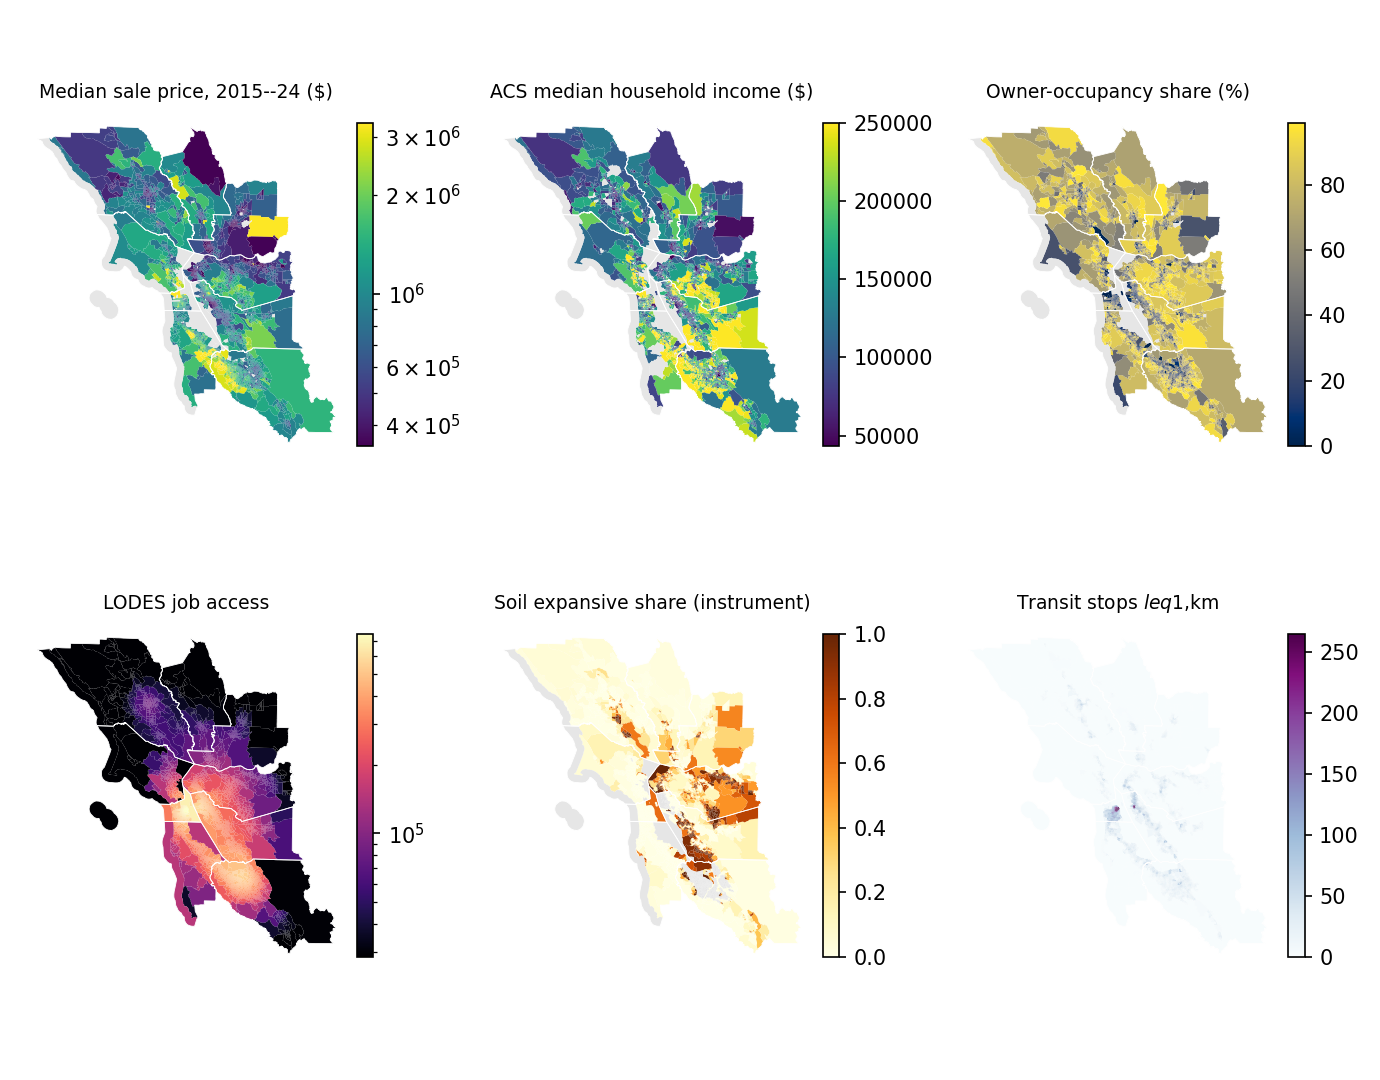
\includegraphics[width=\textwidth]{figures/src_maps.png}
\caption{Block-group choropleths (county boundaries in white): median sale price
(2015--24, CoreLogic), ACS median household income, owner-occupancy share, LODES
job access, SSURGO soil expansive share (the instrument), and transit-stop
density. Colour scales are 2nd--98th percentile; price and job access are log.}
\label{fig:maps}
\end{figure}

% =============================================================================
\section{CoreLogic / Cotality property records (the price spine --- landed)}\label{sec:corelogic}
% =============================================================================
The price/transaction spine has now landed. It was pulled manually from
Stanford Libraries' Redivis ``Data Farm'' (Cotality Smart Data Platform,
formerly CoreLogic) as two Bay-Area-filtered extracts (the nine-county FIPS
filter run server-side); PII columns (owner / buyer / seller names and mailing
addresses) were excluded at query time per the Stanford EULA and IRB rules. The
two tables sit at different grains:
\begin{itemize}[leftmargin=1.5em, itemsep=1pt]
\item \textbf{Owner Transfer (deed)} --- \emph{transaction grain}: \CLNTX{}
  recorded sales spanning \CLYEARMIN--\CLYEARMAX, with sale amount/date, deed and
  sale-type codes, and the resale / new-construction / interfamily / foreclosure-REO
  indicators used to screen for arms-length transactions.
\item \textbf{Property (tax assessor)} --- \emph{parcel grain}: \CLNPARCEL{}
  parcels (\CLNRESPARCEL{} residential), each carrying land use, parcel lat/long,
  assessed land/improvement/total value, annual tax, beds/baths/rooms, living and
  lot square footage, units, stories, foundation type, and owner-occupancy.
\end{itemize}

\paragraph{Merge \& geocoding.} Each parcel is geocoded to a TIGER block group by
its parcel lat/long (98.9\% of parcels carry coordinates), and the deeds are
joined to the parcels on \texttt{CLIP}: \CLMATCHRATE{} of transactions match a
parcel and \CLGEORATE{} carry a block-group \texttt{GEOID}. The outputs are
\path{corelogic/clean/corelogic_transactions_bg.parquet} (one row per sale, with
characteristics + assessed value/tax + \texttt{GEOID}) and
\path{corelogic/clean/corelogic_parcels_bg.parquet} (one row per parcel) --- so
every sale joins straight onto the crosswalk, job access, soil and controls.

\paragraph{First-pass diagnostics (is the data sane?).} The headline analysis
subset --- residential, arms-length, sale year $\geq 1990$, price in
\$10k--\$50M --- is \CLNANALYSIS{} transactions. Tables~\ref{tab:cl-county}
and~\ref{tab:cl-chars} and Figure~\ref{fig:cl} summarize it.

\begin{table}[H]\centering\footnotesize
\setlength{\tabcolsep}{5pt}
\caption{Residential arms-length sales by county (1990--2024).}
\label{tab:cl-county}
\begin{tabular}{lrrrrr}
\toprule
County & Sales & Median & P25 & P75 & Median \$/sqft \\
\midrule
Alameda & 638,761 & \$416,000 & \$233,000 & \$700,000 & \$279 \\
Contra Costa & 641,110 & \$377,000 & \$210,000 & \$625,000 & \$215 \\
Marin & 124,439 & \$627,500 & \$355,500 & \$1,050,000 & \$351 \\
Napa & 61,724 & \$400,000 & \$220,000 & \$646,500 & \$230 \\
San Francisco & 220,049 & \$645,000 & \$340,500 & \$1,075,000 & \$502 \\
San Mateo & 276,116 & \$590,000 & \$329,000 & \$1,005,000 & \$382 \\
Santa Clara & 696,180 & \$520,000 & \$292,000 & \$852,500 & \$326 \\
Solano & 255,577 & \$285,000 & \$165,000 & \$450,000 & \$169 \\
Sonoma & 255,249 & \$350,155 & \$205,000 & \$575,000 & \$225 \\
\midrule
\textbf{All 9 counties} & 3,169,205 & \$435,000 & \$245,000 & \$743,000 & \$273 \\
\bottomrule
\end{tabular}

\end{table}

\begin{table}[H]\centering\footnotesize
\setlength{\tabcolsep}{5pt}
\caption{Residential parcel characteristics (Property file).}
\label{tab:cl-chars}
\begin{tabular}{lrrrrr}
\toprule
Variable & N & Median & Mean & P10 & P90 \\
\midrule
Year built & 1,862,204 & 1,971 & 1,969 & 1,930 & 2,004 \\
Bedrooms & 1,800,324 & 3 & 3 & 2 & 4 \\
Bathrooms & 1,845,982 & 2 & 2 & 1 & 3 \\
Living area (sq ft) & 1,867,953 & 1,594 & 1,812 & 984 & 2,802 \\
Lot size (sq ft) & 1,751,679 & 6,098 & 46,199 & 2,500 & 20,473 \\
Assessed total value & 1,890,940 & \$558,000 & \$764,236 & \$144,284 & \$1,501,236 \\
Annual property tax & 1,888,307 & \$7,581 & \$9,995 & \$2,535 & \$18,991 \\
\bottomrule
\end{tabular}

\end{table}

\begin{figure}[H]\centering
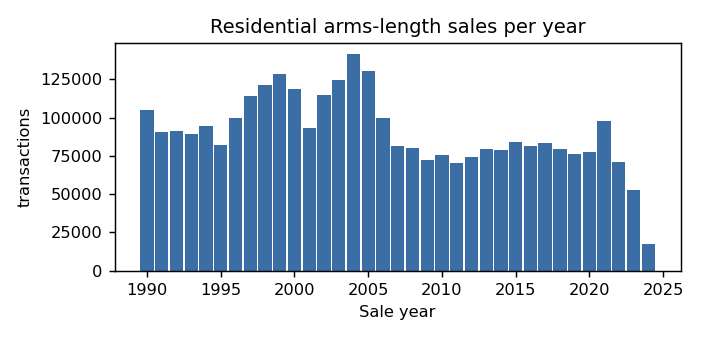
\includegraphics[width=0.49\textwidth]{figures/cl_sales_by_year.png}\hfill
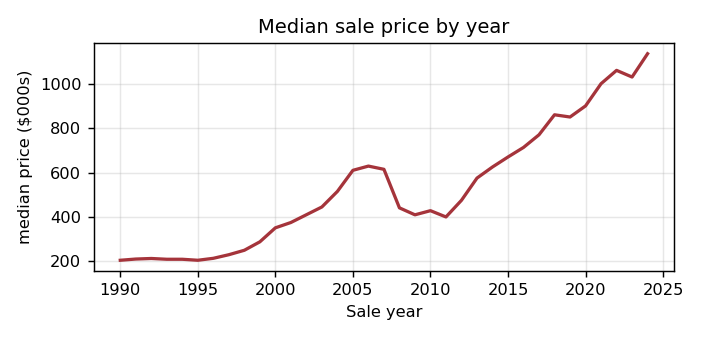
\includegraphics[width=0.49\textwidth]{figures/cl_median_price_by_year.png}\\[3pt]
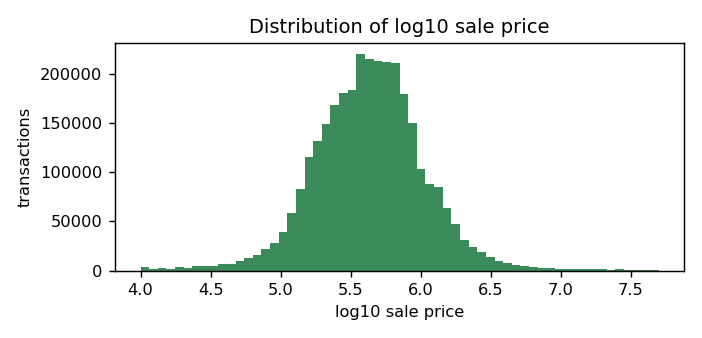
\includegraphics[width=0.49\textwidth]{figures/cl_price_hist.png}\hfill
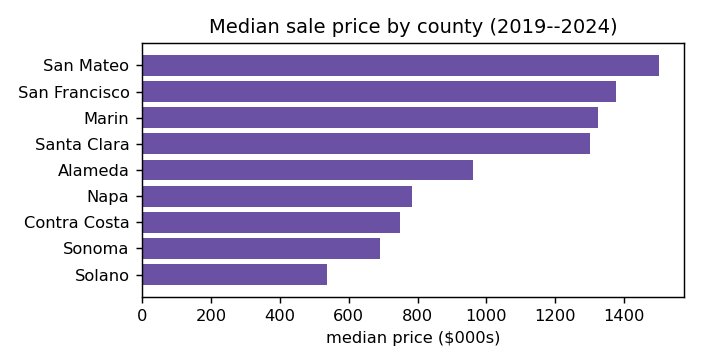
\includegraphics[width=0.49\textwidth]{figures/cl_price_by_county.png}
\caption{CoreLogic diagnostics (residential arms-length subset). Clockwise from
top-left: sales per year, median sale price by year, median price by county
(2019--2024), and the log-price distribution.}
\label{fig:cl}
\end{figure}

\paragraph{Verdict.} The extracts are internally consistent and track external
benchmarks. The median-price-by-year series (Figure~\ref{fig:cl}, top-right)
reproduces the Bay Area cycle --- roughly \$200k in the early 1990s, a $\sim$\$620k
peak in 2006--07, the 2008--11 trough near \$410k, and the 2012--2022 boom past
\$1\,M. The cross-county ordering (Marin / San Francisco / San Mateo / Santa Clara
dear, Solano cheapest), the price-per-square-foot gradient, and the Prop-13-depressed
assessed values (median assessed \$558k at a $\sim$1.2\% effective tax rate) are
all what one expects. This is real signal, not noise --- a sound basis to iterate
the cleaning and arms-length definitions.

% =============================================================================
\section{The instrument pipeline status}\label{sec:instrument}
% =============================================================================
This is the section most relevant to the meeting. The soil instrument is built
in four stages; this run completes the first two and stages the fourth, leaving
a single manual blocker:

\begin{enumerate}[leftmargin=2em]
\item \textbf{SSURGO engineering-property extract --- DONE.}
  \path{mapunit_engineering_properties.parquet} (\NMAPUNITS{} map units)
  holds the depth-weighted shrink-swell / plasticity / bearing properties that
  are the instrument's raw material.
\item \textbf{Map-unit $\to$ block-group aggregation --- DONE (was the open TODO).}
  \path{bg_soil_engineering.parquet} areal-weights the engineering properties
  into the \NSOILBG{} covered block groups, using the SSURGO spatial
  \texttt{MUPOLYGON} polygons (\NSOILPOLY{} polygons, full mukey coverage of the
  tabular extract) intersected with the TIGER block groups in CA-Albers. The soil
  instrument now reaches the estimation geography. This previously-flagged TODO
  is resolved.
\item \textbf{Predicted construction-cost index --- BLOCKED on RS Means
  (the only remaining blocker).}
  Converting engineering properties into a dollar foundation-cost index requires
  the RS Means foundation-cost schedule (slab-on-grade vs.\ pier/pile vs.\ mat),
  a licensed product (Section~\ref{sec:rsmeans}). Until
  \path{foundation_cost_schedule.csv} lands, the index cannot be computed; this
  is documented in \path{soil/derived/TODO_bg_aggregation_and_cost_index.md}
  (whose BG-aggregation half is now marked done).
\item \textbf{Residualization --- STAGED, not estimated.}
  \path{clean/bg_design_matrix.parquet} assembles the block-group covariates
  the demand memo (\S5) residualizes the predicted cost index against --- job
  access, seismic-zone share, open-space distance, transit-stop density (shore
  distance and slope/elevation still to be added). The regression is left as a
  \texttt{TODO} because its dependent variable (the cost index) is blocked on
  RS Means.
\end{enumerate}

% =============================================================================
\section{Manual hand-offs (action required)}\label{sec:manual}
% =============================================================================

\begin{receivedbox}{CoreLogic / Cotality --- price / transaction spine}
\role{the dependent-variable side of demand.}\par\smallskip
\textbf{Status: landed and processed} (Section~\ref{sec:corelogic}). Pulled
manually from \textbf{Stanford Libraries' Redivis ``Data Farm''} (Cotality Smart
Data Platform) as Bay-Area-filtered Owner-Transfer (deed) and Property
(tax-assessor) extracts, PII excluded at query time. Merged on \texttt{CLIP} and
geocoded to block groups (\CLNTX{} transactions, \CLNPARCEL{} parcels).\par
\textbf{Remaining (minor):} the owner-side \emph{user-cost} series still needs an
interest-rate series (e.g.\ FRED 30-yr mortgage) combined with these prices and
the assessed-tax field --- a small automatable follow-up, not a blocker.
\end{receivedbox}

\begin{actionbox}{RS Means --- construction-cost schedule}\label{sec:rsmeans}
\role{converts the SSURGO engineering extract into the predicted foundation-cost
index --- the actual instrument.}\par\smallskip
\textbf{Why manual:} paid subscription product; not scraped.\par
\textbf{Daniel's steps:} pull residential foundation-type cost differentials
(slab-on-grade vs.\ pier/pile vs.\ mat) from RS Means (BU library; else
Questrom).\par
\textbf{Drop path:} \path{data/demand/soil/derived/foundation_cost_schedule.csv}
with columns \texttt{soil\_or\_foundation\_class}, \texttt{usd\_per\_unit\_premium}.\par
\textbf{Note:} published geotechnical cost rules-of-thumb can stand in for a
first pass; default to RS Means for the real index.
\end{actionbox}

\begin{actionbox}{Infutor / Verisk migration --- optional upgrade}
\role{structural moving-cost estimation à la Coven (only if moving costs are
estimated).}\par\smallskip
\textbf{Why manual:} licensed address-history panels.\par
\textbf{Already mitigated:} the free IRS SOI county migration backup was pulled
automatically into \path{data/demand/migration/irs/}. License Infutor/Verisk
only to upgrade; drop under \texttt{data/demand/migration/\{infutor,verisk\}/}.
\end{actionbox}

% =============================================================================
\section{From assembled data to an estimated demand system}\label{sec:nextsteps}
% =============================================================================
Everything above delivers the \emph{inputs} to Layer~I; it does \textbf{not} estimate
demand. No discrete-choice model has been run --- not even a plain conditional logit. This
section is the roadmap from the assembled artifacts to an estimated demand system, and flags
the data inputs still missing. (Estimation and all modeling choices are deliberately left to be
done by hand.)

\subsection{Ingredients: in place vs.\ outstanding}
\begin{center}\footnotesize\setlength{\tabcolsep}{5pt}
\begin{tabular}{p{3.5cm} p{6.0cm} p{4.6cm}}
\toprule
Ingredient & Supplied by & Status \\
\midrule
Agents (household micro) & \path{ca_pums_household/person.parquet} (\texttt{WGTP}-weighted) & \textbf{in place} \\
Location attributes $x_\ell$ & \path{bg_design_matrix} + \path{bg_soil_engineering} + \path{bg_controls} + ACS BG tables & \textbf{in place} \\
Prices / rents & \path{corelogic_transactions_bg.parquet}; ACS gross rent & needs a BG quality-adjusted (hedonic) \textbf{index} \\
Market shares $s_{\ell t}$ & ACS occupied-household counts (\texttt{B25003}) & needs construction once the product is defined \\
Supply-cost instrument & SSURGO soil (BG) + slope/topography & needs RS Means \$ index (blocked); see \S\ref{sec:instrument} \\
Owner user cost & CoreLogic price + assessed tax & needs an interest-rate series (FRED 30-yr) --- small \\
Choice set / products & --- & a \textbf{modeling decision}, not data \\
\bottomrule
\end{tabular}
\end{center}

\subsection{Roadmap}
\begin{enumerate}[leftmargin=1.6em, itemsep=1.5pt]
\item \textbf{Define the product and market.} Unit of choice: block group $\ell$ (baseline), or
  $\ell\times$ structure type (SF/MF), or $\ell\times$ tenure. Market $t$: a pooled cross-section
  (e.g.\ 2019--2023) or a panel. Define the \emph{outside option} (e.g.\ reside outside the region).
\item \textbf{Construct market shares} $s_{\ell t}$ from the ACS occupied-household counts
  (\texttt{B25003}) consistent with the product definition; the denominator (market size) fixes the
  outside-option share.
\item \textbf{Build the price/rent index.} From CoreLogic, a BG-level \emph{hedonic} sale-price
  index controlling for beds/baths/sq\,ft/year-built; for renters, ACS gross rent (\texttt{B25064})
  or CoreLogic rentals; for owners, convert price to a \emph{user cost} (price $+$ property tax $+$
  an interest-rate series).
\item \textbf{Specify utility.} $\delta_\ell = x_\ell\beta - \alpha\,\text{price}_\ell + \xi_\ell$,
  with the agglomeration term $w(N)$ and the density disamenity $g(D_\ell)$ entered explicitly;
  random coefficients drawn over the PUMS demographic distribution.
\item \textbf{Estimate, baseline $\to$ structural.} (a) a plain conditional logit as a transparent
  first pass (note IIA); (b) BLP random coefficients via Berry inversion $+$ PUMS micro-moments
  (income$\times$price, income$\times$job-access, family$\times$bedrooms, tenure$\times\cdots$).
\item \textbf{Instrument the price.} Price is correlated with unobserved location quality $\xi_\ell$.
  Supply-cost shifters: the SSURGO soil foundation-cost instrument (once RS Means gives the dollar
  index) and slope/topography (Saiz tradition); plus BLP differentiation instruments
  (Gandhi--Houde). Exclusion: soil affects sorting \emph{only} through construction cost,
  residualized against the seismic / open-space / slope channels already collected as controls.
\item \textbf{Micro-moments.} Match the joint distribution of household demographics $\times$
  chosen-location attributes (PUMS agents) to pin the random coefficients.
\item \textbf{(For counterfactuals, not demand alone) the supply equation.} $H_\ell$ as a function
  of $\bar z_j$ and construction cost (RS Means $+$ permits) closes the equilibrium the preemption
  counterfactuals need.
\end{enumerate}

\subsection{Remaining data inputs}
\begin{itemize}[leftmargin=1.5em, itemsep=1pt]
\item \textbf{RS Means} construction-cost schedule --- the soil instrument's dollar form; the one
  blocker (\S\ref{sec:manual}).
\item \textbf{Interest-rate series} (e.g.\ FRED 30-yr mortgage) for the owner user cost --- small,
  automatable.
\item \textbf{(Layer II / III, separate)} permits for the supply equation; the multi-jurisdiction
  discretionary-review ($\tau_j$) panel and the by-right envelope ($\bar z_j$) for the regulation game.
\end{itemize}

\subsection{Tooling}
The artifacts are already close to the \texttt{(product\_data, agent\_data)} shape \texttt{pyblp}
(Conlon \& Gortmaker) expects --- one row per product$\times$market with shares, prices,
characteristics, and instruments; PUMS as weighted agents. A conditional-logit first pass needs
only the product table.

% =============================================================================
\section{Reproducibility}
% =============================================================================
\begin{itemize}[leftmargin=1.5em]
\item \textbf{Geographic scope:} FIPS \texttt{06001, 06013, 06041, 06055, 06075,
  06081, 06085, 06095, 06097}; national/statewide sources are filtered to these.
\item \textbf{Manifest:} \path{data/demand/_manifest.csv} --- columns
  \texttt{source}, \texttt{url}, \texttt{local\_path}, \texttt{bytes},
  \texttt{sha256}, \texttt{fetched\_at}, \texttt{status}; rows keyed by
  (source, path) so re-runs update in place.
\item \textbf{Paths:} \path{demand_estimation/demand_paths.py} imports
  \texttt{DATA\_ROOT} from the minutes pipeline's \texttt{paths.py}; respects
  \texttt{MFHR\_DATA\_ROOT}. No absolute paths are hard-coded.
\item \textbf{Dependencies added:} \texttt{pyarrow}, \texttt{pyogrio} (bundles
  GDAL), \texttt{shapely}, \texttt{us} (see \texttt{requirements.txt} /
  \texttt{environment-notes.md}).
\item \textbf{One command:} \texttt{python -m demand\_estimation.build}
  (idempotent, resumable, failure-isolated per source).
\end{itemize}

% =============================================================================
\section{Definition-of-done checklist}
% =============================================================================
\newcommand{\yes}{\textcolor{green!55!black}{\checkmark}}
\newcommand{\no}{\textcolor{red}{\ding{55}}}
\newcommand{\partialmark}{\textcolor{orange!90!black}{$\circ$}}

\begin{itemize}[leftmargin=2.2em, itemsep=2pt]
\item[\yes] Every \S2 source downloaded, checksummed (\texttt{sha256}), and
  logged in \texttt{\_manifest.csv}.
\item[\yes] BG$\leftrightarrow$jurisdiction crosswalk built (\NBG{} block
  groups $\to$ \NJURIS{} jurisdictions) --- the load-bearing artifact.
\item[\yes] Soil engineering-property extract built (\NMAPUNITS{} map units),
  \textbf{and} the map-unit$\to$block-group areal-weighted aggregate
  (\texttt{bg\_soil\_engineering.parquet}, \NSOILBG{} BGs) from \NSOILPOLY{}
  SSURGO spatial polygons (full mukey coverage). Only the RS Means cost-index
  join remains, as a documented \texttt{TODO}.
\item[\yes] Hazard + amenity controls staged for residualization
  (\texttt{bg\_controls.parquet}: seismic-zone share, open-space distance,
  transit-stop density).
\item[\yes] ACS micro (\NPUMSHH{} CA households) + BG tables (8 table groups)
  staged for BLP.
\item[\yes] IRS migration pulled; Infutor/Verisk stubbed.
\item[\yes] Every \S3 manual source has a \texttt{\_stubs/<name>/README.md} +
  manifest row (CoreLogic, RS Means, Infutor/Verisk).
\item[\yes] CoreLogic/Cotality price spine \textbf{landed \& processed}
  (\CLNTX{} sales, \CLNPARCEL{} parcels, merged + geocoded to BG, sanity-checked);
  RS Means remains the one outstanding licensed blocker.
\item[\yes] 511 regional transit: key \textbf{present} $\Rightarrow$ all-operator
  bundle (\NSTOPS{} stops) fetched; full measure \path{transit_stops_1km_all}
  (\NTRANSITBG{} BGs) built, with the BART+Caltrain baseline
  (\path{transit_stops_1km_bartcaltrain}) retained for auditability.
\item[\yes] \texttt{demand\_data\_report.tex} compiled to PDF, zero undefined
  references.
\item[\yes] Nothing behind auth was scraped or circumvented; no credentials
  fabricated (CGS regulatory layer pulled from its public copy; 511 transit
  fetched with the supplied key; CoreLogic/RS Means stubbed, not sourced).
\end{itemize}

\noindent\partialmark{} \emph{Single remaining soil blocker:} only the predicted
construction-cost index (needs the RS Means schedule) is outstanding; the
map-unit$\to$block-group aggregation TODO from the first run is now resolved ---
see Section~\ref{sec:instrument}.


\end{document}
